\Chapter{Titkosítási algoritmusok}

A bemutatott programoknál szó esett titkosítási algoritmusokról, ez eltér az eljárásoktól, amiket adattitkosítási módszereknek neveztem. Egy titkosítási algoritmus olyan matematikai folyamat, amely egy szimpla szöveget (plain text) kódolt szöveggé transzformál (cipher text).
\\ Lehet szimmetrikus vagy aszimmetrikus egy algoritmus, ez a kódolt szöveg és a titkosítási kulcs(ok) közötti kapcsolatot írja le.
\vspace{5pt}\\Mindegyik titkosítási módszer, legyen az adatbázis titkosítás, vagy fájlrendszer titkosítás, valamilyen titkosítási algoritmust alkalmaz.
\\A dolgozat méréseit és összehasonlításait ezeken az algoritmusokon végeztem.
\vspace{5pt}\\Az algoritmusok belső matematikai működéséről részletes leírást nem tartalmaz a dokumentum. Bonyolultak és hosszúak, sok-sok oldalt kellene írni ahhoz, hogy megismerjük minden egyes algoritmus pontosan milyen számításokat végez a végső kódölt szöveg eléréséhez.
 
\Section{Szimmetrikus titkosítási algoritmusok} 
\noindent - Adat titkosítására és dekódolására egy privát kulcsot használ.
\\- Az adatok megosztásához a címzettnek rendelkeznie kell a visszafejtési kulcs másolatával. Ez a titkosítás legegyszerűbb, legrégebbi és legismertebb fajtája.
\\- Hátránya a kulcs megosztásából ered, ha a visszafejtési kulcs publikussá válik, az adatszivárgáshoz (data leak) vezethet.
\\- Előnye a sebesség. \newline

\begin{figure}[h]
	\centering
	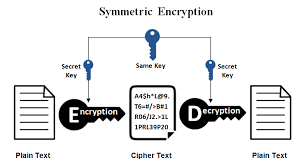
\includegraphics[scale=0.7]{images/sym.png}
	\caption{Szimmetrikus titkosítási algoritmusok működése.}
	\label{fig:sym_encryptino}
\end{figure}

\subsection{AES (Advanced Encryption Standard)}
\noindent - Bevált, megbízható titkosítási módszer. 
\vspace{5pt}\\- Komplex, több fázisból álló matematikai számításokat hajt végre.
\vspace{5pt}\\- Hátránya, hogy szoftveresen nehezen implementálható lehet, illetve komplexitása és nagysága miatt teljesítményi ideje is nagy.
\vspace{5pt}\\- Úgynevezett block cipher, azaz blokk titkosítás. Blokkok mérete 128 bit.
\vspace{5pt}\\- 3 fajtája van:
\\AES-128 – 128 bit nagyságú titkosítási kulcsot alklamaz.
\\AES-192 – 192 bit nagyságú titkosítási kulcsot alkalmaz.
\\AES-256 – 256 bit nagyságú titkosítási kulcsot alkalmaz.
\vspace{5pt}\\- Számítást bájtokon nem pedig biteken végez. 128 bites blokkot az algoritmus 16 bájtként kezel. Ezt a 16 bájtot 4 sorba és oszlopba rendezi a mátrixműveletekhez.
\vspace{5pt}\\- Kulcs méretétől függ, hogy hány kört fog az algoritmus elvégezni. 128 bites kulcs – 10 kör, 192 bites kulcs – 12 kör, 256 bites kulcs – 14 kör.
\vspace{5pt}\\- Mindegyik kör egy másik 128 bites kulcsot használ, amit az eredeti AESkulcsból számolnak ki.



\subsection{DES (Data Encryption Standard)}
\noindent - Block cipher, egy blokk 64 bit nagyságú.
\vspace{5pt}\\- 64 bit nagyságú sima szöveg titkosítás után 64bit nagyságú titkosított szöveget eredményez.
\vspace{5pt}\\- 16 sorozatot véget el matematikai számításokból, mindegyikhez külön titkosítási kulcsot használ.
\vspace{5pt}\\- Kulcsok mérete 56 bit (64 bit, de 8-at közülük nem használ).
\vspace{5pt}\\- Hátránya lehet, hogy a titkosítás és visszafejtés ugyanazzal az algoritmussal és kulcsokkal történik.
\vspace{5pt}\\- Feistel kódon alapul.



\subsection{Triple DES}
\noindent- Működése megegyezik a DES működésével.
\vspace{5pt}\\- 3x16 sorozatot végez, így biztonságosabbnak mondható.
\vspace{5pt}\\- Hátránya lehet, hogy a titkosítás és visszafejtés ugyanazzal az algoritmussal és kulcsokkal történik.



\subsection{Blowfish}
\noindent - Block cipher, 64 bit méretű blokkok.
\vspace{5pt}\\- Kulcsok mérete 32 bittől 448 bit-ig terjed, változó méretűek, így lehetőséget nyújt személyes és ipari felhasználásra is. Úgynevezett alkulcsokat is használ (subkey), számszerint 18-at. Ez a P tömb.
\vspace{5pt}\\- Sokkal gyorsabb mint a DES és Triple DES.









\newpage \Section{Aszimmetrikus titkosítási algoritmusok}
\noindent - Egy privát és egy publikus kulcsot használ.
\vspace{5pt} \\- A publikus kulcs lehetővé teszi, hogy bárki titkosítsa az adatokat.
\vspace{5pt} \\- A privát kulcs szükséges az adatok  dekódolásához. 
\vspace{5pt} \\- Biztonságosabbnak vélhető, mivel a privát kulcsok nem kerülnek megosztásra, de ugyanakkor nagyobb a számítási költsége is.\newline

\begin{figure}[h]
	\centering
	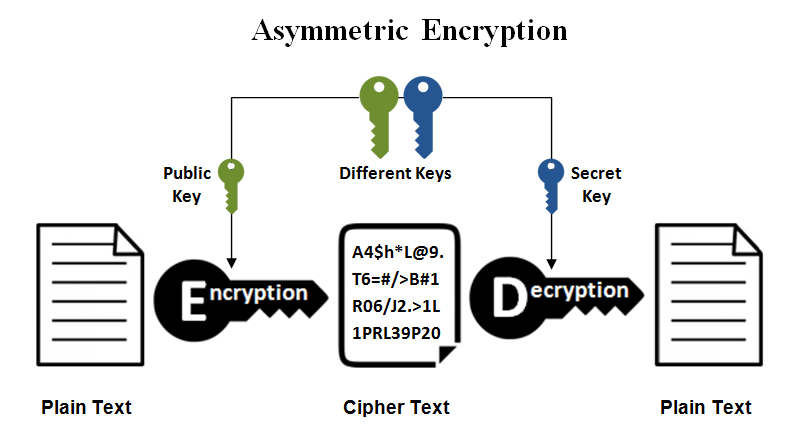
\includegraphics[scale=0.4]{images/asym.png}
	\caption{Aszimmetrikus titkosítási algoritmusok működése.}
	\label{fig:asym_encryptino}
\end{figure}

\subsection{RSA (Rivest–Shamir–Adleman)}
\noindent - Azon az elven alapul, hogy a nagy számok szorzása könnyű, de a nagy számok tényezőkre bontása nehéz. 
\vspace{5pt}\\- A publikus kulcs két számból áll, ami közül az egyik két nagy prímszám szorzata.
\vspace{5pt}\\- A privát kulcs egyik száma ugyanennek a két prímnek a szorzata.


\subsection{DSA (Digital Signature Algorithm)}
\noindent-Digitális aláírások titkosítására használt szabvány. Digitális üzenet hitelesítésére is alkalmas.
\vspace{5pt}\\- Moduláris exponenciáláson (modular exponentiation) alapul, a diszkrét logaritmus (discrete logarithm) problémájával együtt.
\vspace{5pt}\\- Privát kulcsot egy üzenet digitális aláírásárának generálására használják. Ellenőrizni az aláíró publikus kulcsával lehetséges.


\subsection{ECC (Elliptic Curve Cryptography)}
\noindent- RSA-val vetélkedő aszimmetrikus titkosítási módszer.
\vspace{5pt}\\- Kulcs generálása matematikai elliptikus görbék segítségével történik.
\vspace{5pt}\\- „Véges mező feletti sík görbe, amely az egyenletet kielégítő pontokból áll: y²=x³ + ax + b.”
\vspace{5pt}\\- Alapvető kulcs méret 256 bit, de görbétől függően változhat.

\newpage \Section{Hash, hashelés, hash algoritmusok}
A titkosítási módszerek közül kimaradt, az úgynevezett hashing, vagy hashelés. Nem sorolható kimondottan sem az adatbázis sem a fájlrendszerek titkosításához. 
\vspace{5pt} \\Érzékeny adatok tárolására használják, mint a jelszavak.
\vspace{5pt} \\Egyediek és ismételhetőek, ami azt jelenti, hogy egy szó ugyanazzal a hash algoritmussal transzformálva ugyanazt a titkosított szöveget fogja eredményezni. 
\vspace{5pt} \\Egy algoritmus mindig ugyanolyan méretű kimenetet állít elő. 
\vspace{5pt} \\Nagyon nehéz két olyan különböző szót találni, amelyek ugyanazon hash algoritmussal transzformálva ugyanazt a titkosított szöveget eredményeznék.
\vspace{5pt} \\Egy hash algoritmussal transzformált szöveget visszaalakítani egyszerű, értelmes szöveggé (plain text) már nem lehet, éppen ezért használják jelszavak titkosítására.
\vspace{5pt} \\Nem visszaalakíthatósága miatt egyezőség vizsgálatát lehet megnézni két ugyanazon hash algoritmussal transzformált , kódolt szöveg között. Ha két hash egyezik, akkor ugyan az volt a bemeneti érték, ha nem egyeznek, akkor különbözőek voltak.
\vspace{5pt} \\Úgynevezett salt és pepper –rel szokás a hasheket ellátni, magasabb biztonság elérése érdekében.
\vspace{5pt} \\ \underline{Salt:} A titkosítandó szövegrészhez extra szöveg csatolása bonyolultság növeléséhez. Regisztrációkor lehet például az email címet és jelszót kombinálni, majd a kombinált szövegen elvégezni a hash algoritmust. Ilyen adatokat salted hashnek nevezik.
\vspace{5pt} \\ \underline{Pepper:} Salted hash adathoz , tehát már titkosított adathoz fűz további értékeket. Egy adatbázis esetébe ez általában megegyező értéket jelent, azaz minden hashelt adathoz ugyanaz a pepper érték lesz hozzáadva.
\vspace{25pt} \\ Két leggyakrabban implementált hash algoritmus:

\subsection{MD5 (Message Digest 5)}
Régebben gyakran használt funkció, ami egy 128 bites kimenetet állít elő.
\vspace{5pt} \\Kiderült róla, hogy nem ütközésálló (collision resistant), emiatt kriptográfusok más hash algoritmusokat ajánlanak. Egy hash függvényre akkor mondjuk, hogy ütközésálló, hogyha nehéz olyan két különböző bemenetet találni, amely ugyanazt a kimenetet eredményezi.


\subsection{SHA (Secure Hashing Algorithm) Family}
Hat különböző hash függvényből áll: SHA-0, SHA-1, SHA-224, SHA-256, SHA-384, SHA-512.
\vspace{5pt} \\Változó méretű bemenetet alakítanak fix méretű kiementté.
\vspace{5pt} \\Az első négy 512 bites blokkokat használ 32 bites szavakra osztva, az utolsó kettő pedig 1024 bites blokkokat 64 bites szavakra bontva.
\vspace{5pt} \\Kimenet mérete SHA-0 és 1 esetén 160 bit, SHA-224 esetén 224 bit, SHA-256 esetén 256 bit, SHA-384 esetén 384 bit, SHA-512 esetén 512 bit nagyságú.
\vspace{5pt} \\Mindegyik algoritmus hasonlóképpen működik.
\vspace{5pt} \\Eredmény mindig 160 bit hosszú. Eredeti üzenet hosszának kevesebbnek kell lennie, mint $2^{64}$-en bit.
\vspace{5pt} \\A SHA-2 családot, aminek a 256, 384, 512 is a tagja, szélés körben implementálták biztonsági alkalmazásokban és protokollokban, mint a TLS, SSL, PGP, stb.
\vspace{5pt} \\A SHA-256-ot a Debian szoftvercsomag hitelesítésére használják és DKIM üzenetaláírási standard. Linux és Unix gyártók 256 és 512 bites SHA-2 használatára tértek át a biztonságos jelszótároláshoz.
\vspace{5pt} \\Számos kriptovaluta, köztük a Bitcoin is használja a SHA-256-ot.


\vspace{25pt}
\Section{Mérések, összehasonlítások}

A mérések végzéséhez az alkalmazásomból elmentett adatokat fogom tesztadatként használni. Az adatokat struktúrált xml dokumentum formátumban kerülnek tárolásra az összehasonlítások elvégzése érdekében. Három különböző méretű fájlt vizsgálunk. Reális méretű fájlok használatára törekedtem (~500KB, ~2MB ~4MB). Már a 4 MB nagyság (nem titkosított) elérését a program rendeltetésszerű használata esetén is elég valószínűtlen tartom, mivel nagyon sok random adatot kellett bemásoljak ahhoz, hogy elérjem ezt a fájlméretet. 
\vspace{5pt}\\Feltehető a mérési eredmények arányos növekedése nagyobb fájlméret esetén.

\subsection{Tesztprogram}
\vspace{5pt}\noindent A mérések összeállítása előtti próbálgatásaimból megtudtam, hogy a titkosítási és visszafejtési idő (a program kód alapján, a System.currentTimeMillis() parancs használatával) nem mindig egyezik meg ugyanazon fájl többszöri titkosítása esetén. Ebből következik, hogy egy adott fájl titkosítását mindegyik algoritmus használatakor többször is el kell végeznem, hogy egy korrekt közelítő értéket kapjak.
\vspace{5pt}\\A tesztprogram elkészítésére elsősorban a javax.crypto és java.security könyvtárakat használtam. A program szempontjából ezen könyvtárak által szolgáltatott fontosabb \underline{interface-ek}:
\vspace{5pt}\\-Key: Az összes kulcs legfelső szintű interface-e. Meghatározza az összes kulcs objektum által használt funkciókat.
\vspace{5pt}\\-PrivateKey: Célja, hogy csoportosítsa az összes privát kulcs interface-t. Nem tartalmaz metódusokat vagy konstansokat. Speciális privát kulcs interface-ek kiterjesztik ezt az interface-t. 
\vspace{5pt}\\-PublicKey: Célja, hogy csoportosítsa az összes nyilvános kulcs interface-t. Nem tartalmaz metódusokat vagy konstansokat. Speciális nyilvános kulcs interface-ek kiterjesztik ezt az interface-t. \newline

\noindent \underline{Osztályok}:
\vspace{5pt}\\-SecretKeySpec: Használható titkos kulcs létrehozására byte tömbből anélkül, hogy SecretKeyFactory-t kellene hozzá használni. ’Nyers’ titkosítási kulcsok számára különösen hasznos, amelyek ábrázolhatók byte tömbként és nincs hozzájuk kulcsparaméter társítva.
\vspace{5pt}\\-KeyPair: Egy kulcspár (egy nyilvános és egy privát kulcs) egyszerű tárolója.
\vspace{5pt}\\-KeyGenerator: Egy titkos (szimmetrikus) kulcsgenerátor funkcionalitását biztosítja.
\vspace{5pt}\\-KeyPairGenerator: Nyilvános és privát kulcspárok létrehozására szolgál.
\vspace{5pt}\\-Cipher: Kriptográfiai titkosítási funkciókat biztosít titkosításhoz és visszafejtéshez. A Java Cryptographic Extension (JCE) keretrendszer magját képzi. \newline

\vspace{10pt} \noindent A tesztprogram felépítése hasonló szimmetrikus és aszimmetrikus titkosítás esetén is, néhány eltéréssel.
\\A tesztprogram teljesen reprodukálható a felsorolt osztályok és interface-ek használatával.
\vspace{5pt}\\ Lényegi különbség a két alkalmazás között (szimmetrikus és aszimmetrikus) a kulcsok méretében, létrehozásában / generálásában rejlik. A kódrészletekbe nem megengedett az ékezetes betűk használata, ezért ékezet nélkül kerültek bele magyar szavak.
\vspace{5pt}\\ - Fájl elérési útvonal, jelen esetben a vizsgált xml fájlok útvonala, amik a tesztek készítésekor az asztalomon voltak.
\begin{java}
String filePath = "C:\\Users\\AMD\\Desktop\2MB.xml";
File inputFile = new File(filePath);
\end{java}
\vspace{5pt}- Az objektum és metódus, ami a titkosítást és dekódolást végzi. Az implementálás RSA esetén így nézett ki:
\begin{java}
//Titkositas
Cipher cipher = Cipher.getInstance("RSA");
cipher.init(Cipher.ENCRYPT_MODE, publicKey);
byte[] encryptedFileBytes = cipher.doFinal(inputBytes);

//Visszafejtes
cipher.init(Cipher.DECRYPT_MODE, privateKey);
byte[] decryptedFileBytes = cipher.doFinal(inputBytes);
\end{java}
Szimmetrikus algoritmus használata esetén a publicKey és privateKey helyére a létrehozott szimmetrikus kulcsot kell elhelyezni.
\vspace{15pt}\\ - Kódolt byte-ok fájlba írása, majd a dekódolt byte-ok másik fájlba írása. Azért dekódoltam, hogy meggyőződjek róla, hogy semmi hiba nem történt titkosítás és visszafejtés alatt.
\begin{java}
//Titkositott byte-ok irasa
FileOutputStream outputStream = 
			new FileOutputStream(encryptedFile);
outputStream.write(encryptedFileBytes);
	
//Dekodolt byte-ok irasa
outputStream = new FileOutputStream(decryptedFile);
outputStream.write(decryptedFileBytes);
	
//Ezek lezarasa a megfelelo helyen
outputStream.close();
inputStream.close();
\end{java}
\vspace{5pt}- Az eltelt idő mérésére az említett System.currentTimeMillis() funkció:
\begin{java}
//Kezdo ertek
long start = System.currentTimeMillis();
//Vegso ertek
long end = System.currentTimeMillis();	
//Korrekt idotartam megkapasa
long finalTime = end2-start2;	
\end{java}
A kezdő és végérték inicializálását a megfelelő helyekre kell elhelyezni. Titkosítás és visszafejtés esetén is a kezdőértéket a Cipher objektum létrehozása elé raktam, a kulcs létrehozását nem számítottam bele az időbe. A végértéket a titkosított/dekódolt byte-ok fájlba történő írása után.
\vspace{15pt} \\Ahol a legnagyobb a kód különbsége, a kulcsok létrehozása. Először is meg kell jegyezzem, hogy két módon lehet megfelelő kulcsokat létrehozni:
\vspace{5pt}\\ A megfelelő generátor objektummal (szimmetrikus - KeyGenerator, aszimmetrikus - KeyPairGenerator).
\vspace{5pt}\\ Létrehozni egy String-et, majd abból egy Key objektumot a SecretKeySpec osztály segítségével.
\vspace{5pt}\\Az aszimmetrikus algoritmusok méréséhez az első verziót alkalmaztam, a szimmetrikus algoritmusokhoz pedig a másodikat.
\vspace{5pt}\\ \noindent -Szimmetrikus algoritmus méréseknél a kulcs létrehozása a következő módon nézett ki DES használata esetén:
\begin{java}
String key = "T@stK#Y1";
//Titkos kulcs letrehozasa
Key secretKey = new SecretKeySpec(key.getBytes(), "DES");	
\end{java}
Az alkalmazás többi részében a secretKey objektumot kellett használni.
\vspace{7pt}\\- Aszimmetrikus algoritmusok mérésekor a következő volt a kód:
\begin{java}
KeyPairGenerator generator = 
			KeyPairGenerator.getInstance("RSA");
generator.initialize(2048);
KeyPair pair = generator.generateKeyPair();
	
PrivateKey privateKey = pair.getPrivate();
PublicKey publicKey = pair.getPublic();
\end{java}
Titkosításhoz a publicKey-t kell használni, visszafejtéshez pedig a privateKey-t.


\subsection{Eredmények, következtetések}
A számítógépem paraméterei:
\\ Processzor - AMD Ryzen 5 3600X 6-Core 3.79GHz
\\ RAM - 16 GB
\\ OS - Windows 10 Home 64 - bit

\vspace{10pt} \noindent \underline{Ismertetett szimmetrikus titkosítási algoritmusok összehasonlítása:}

\begin{center}
	
	
	\begin{tabular}{|p{2.4cm}|p{2.7cm}|p{2.7cm}|p{2.7cm}|p{2.7cm}|}
		\hline
		 & \textbf{AES} & \textbf{DES} & \textbf{Triple DES}  & \textbf{Blowfish} \\
		\hline
		Lehetséges kulcs méret(ek) & 128/192/256 bit & 64 bit (56-ot használ) & Összesen 168 bit & Mérete 32 bittől 448 bitig terjedhet \\
		\hline
		Mekkora egy block mérete? & 128 bit & 64 bit & 64 bit & 64 bit \\
		\hline
		Hány kört végez az algoritmus? & Kulcs méretétől függ  & 16 kör & 3 x 16 kör & 16 kör \\
		 & 128 bit - 10 kör & & & \\
		 & 192 bit - 12 kör & & & \\
		 & 256 bit - 14 kör & & & \\
		\hline
		Külön kulcsot használ-e minden körben? & Igen, mindegyik kör más kulcsot használ. & Igen, különböző 48 bites kulcsokat. & Három különböző DES kulcsot. & Igen, 32 bit nagyságúakat. \\
		\hline
		Sikerült-e már feltörni? & Nem. & Igen, úgynevezett brute force támadással. & Vegyes válaszokat találtam, de mivel már nem igazán használják csak régebbi szoftverek, és a DES is fel lett törve, ezért valószínűleg \textbf{igen}. & Nem. \\
		\hline
	\end{tabular}
\end{center}
Úgy gondolom, hogy az algoritmusok biztonságával kapcsolatosan megfelelő méréseket nem tudok végezni, ezért nem szerepelnek a dokumentumban. A táblázat ’Sikerült-e már feltörni’ sorában lévő információk is az interneten talált adatok.\newline

\newpage
\noindent Az AES algoritmusok 128 bit nagyságú kulcsot használtak. A táblázatokban szereplő értékek milliszekundumban (ms) értendők.
\begin{center}
	\begin{tabular}{|p{2.4cm}|p{2cm}|p{2cm}|p{2cm}|p{2cm}|}
		\hline
		\textbf{Titkosítás} \newline \textbf{500KB} & \textbf{AES} & \textbf{DES} & \textbf{Triple DES} & \textbf{Blowfish}\\
		\hline
		\textbf{1.mérés} & 49 & 51 & 73 & 48\\
		\hline
		\textbf{2.mérés} & 44 & 50 & 69 & 44\\
		\hline
		\textbf{3.mérés} & 46 & 50 & 70 & 49\\
		\hline
		\textbf{4.mérés} & 43 & 50 & 74 & 49\\
		\hline
		\textbf{5.mérés} & 48 & 56 & 71 & 46\\
		\hline
		\textbf{6.mérés} & 46 & 57 & 74 & 50\\
		\hline
		\textbf{7.mérés} & 44 & 53 & 74 & 52\\
		\hline
		\textbf{8.mérés} & 44 & 57 & 74 & 52\\
		\hline
		\textbf{9.mérés} & 47 & 58 & 70 & 50\\
		\hline
		\textbf{10.mérés} & 61 & 58 & 70 & 46\\
		\hline
		\hline
		\textbf{Átlag} & \textbf{46,2} & \textbf{54} & \textbf{71,9} & \textbf{48,6}\\
		\hline
	\end{tabular}
\end{center}

\begin{center}
	\begin{tabular}{|p{2.4cm}|p{2cm}|p{2cm}|p{2cm}|p{2cm}|}
		\hline
		\textbf{Visszafejtés} \newline \textbf{500KB} & \textbf{AES} & \textbf{DES} & \textbf{Triple DES} & \textbf{Blowfish}\\
		\hline
		\textbf{1.mérés} & 7 & 17 & 28 & 14\\
		\hline
		\textbf{2.mérés} & 7 & 21 & 28 & 13\\
		\hline
		\textbf{3.mérés} & 6 & 17 & 29 & 12\\
		\hline
		\textbf{4.mérés} & 7 & 16 & 35 & 13\\
		\hline
		\textbf{5.mérés} & 7 & 17 & 28 & 13\\
		\hline
		\textbf{6.mérés} & 7 & 18 & 35 & 12\\
		\hline
		\textbf{7.mérés} & 8 & 16 & 33 & 14\\
		\hline
		\textbf{8.mérés} & 6 & 20 & 29 & 15\\
		\hline
		\textbf{9.mérés} & 8 & 17 & 29 & 14\\
		\hline
		\textbf{10.mérés} & 8 & 19 & 30 & 14\\
		\hline
		\hline
		\textbf{Átlag} & \textbf{7,2} & \textbf{17,8} & \textbf{30,4} & \textbf{13,4}\\
		\hline
	\end{tabular}
\end{center}

\newpage
\begin{center}
	\begin{tabular}{|p{2.4cm}|p{2cm}|p{2cm}|p{2cm}|p{2cm}|}
		\hline
		\textbf{Titkosítás} \newline \textbf{1MB} & \textbf{AES} & \textbf{DES} & \textbf{Triple DES} & \textbf{Blowfish}\\
		\hline
		\textbf{1.mérés} & 55 & 70 & 105 & 60\\
		\hline
		\textbf{2.mérés} & 51 & 63 & 98 & 65\\
		\hline
		\textbf{3.mérés} & 57 & 68 & 109 & 57\\
		\hline
		\textbf{4.mérés} & 58 & 67 & 102 & 58\\
		\hline
		\textbf{5.mérés} & 55 & 68 & 110 & 62\\
		\hline
		\textbf{6.mérés} & 54 & 71 & 106 & 58\\
		\hline
		\textbf{7.mérés} & 53 & 63 & 102 & 59\\
		\hline
		\textbf{8.mérés} & 57 & 65 & 105 & 64\\
		\hline
		\textbf{9.mérés} & 51 & 70 & 107 & 53\\
		\hline
		\textbf{10.mérés} & 51 & 72 & 100 & 56\\
		\hline
		\hline
		\textbf{Átlag} & \textbf{54,2} & \textbf{67,7} &\textbf{ 104,4} & \textbf{59,2}\\
		\hline
	\end{tabular}
\end{center}

\begin{center}
	\begin{tabular}{|p{2.4cm}|p{2cm}|p{2cm}|p{2cm}|p{2cm}|}
		\hline
		\textbf{Visszafejtés} \newline \textbf{1MB} & \textbf{AES} & \textbf{DES} & \textbf{Triple DES} & \textbf{Blowfish}\\
		\hline
		\textbf{1.mérés} & 13 & 29 & 59 & 18\\
		\hline
		\textbf{2.mérés} & 12 & 30 & 58 & 21\\
		\hline
		\textbf{3.mérés} & 11 & 30 & 68 & 18\\
		\hline
		\textbf{4.mérés} & 12 & 31 & 58 & 19\\
		\hline
		\textbf{5.mérés} & 12 & 30 & 59 & 21\\
		\hline
		\textbf{6.mérés} & 12 & 31 & 58 & 18\\
		\hline
		\textbf{7.mérés} & 12 & 32 & 59 & 20\\
		\hline
		\textbf{8.mérés} & 11 & 29 & 59 & 20\\
		\hline
		\textbf{9.mérés} & 12 & 27 & 59 & 18\\
		\hline
		\textbf{10.mérés} & 13 & 30 & 56 & 19\\
		\hline
		\hline
		\textbf{Átlag} & \textbf{12} & \textbf{29,9} & \textbf{59,3} & \textbf{19,2}\\
		\hline
	\end{tabular}
\end{center}

\newpage
\begin{center}
	\begin{tabular}{|p{2.4cm}|p{2cm}|p{2cm}|p{2cm}|p{2cm}|}
		\hline
		\textbf{Titkosítás} \newline \textbf{2MB} & \textbf{AES} & \textbf{DES} & \textbf{Triple DES} & \textbf{Blowfish}\\
		\hline
		\textbf{1.mérés} & 52 & 86 & 149 & 71\\
		\hline
		\textbf{2.mérés} & 58 & 85 & 148 & 68\\
		\hline
		\textbf{3.mérés} & 51 & 90 & 157 & 65\\
		\hline
		\textbf{4.mérés} & 56 & 86 & 149 & 66\\
		\hline
		\textbf{5.mérés} & 51 & 85 & 145 & 71\\
		\hline
		\textbf{6.mérés} & 60 & 97 & 161 & 76\\
		\hline
		\textbf{7.mérés} & 55 & 86 & 166 & 69\\
		\hline
		\textbf{8.mérés} & 60 & 95 & 153 & 68\\
		\hline
		\textbf{9.mérés} & 70 & 89 & 157 & 70\\
		\hline
		\textbf{10.mérés} & 54 & 87 & 154 & 74\\
		\hline
		\hline
		\textbf{Átlag} & \textbf{56,7} & \textbf{88,6} & \textbf{153,9} & \textbf{69,8} \\
		\hline
	\end{tabular}
\end{center}

\begin{center}
	\begin{tabular}{|p{2.4cm}|p{2cm}|p{2cm}|p{2cm}|p{2cm}|}
		\hline
		\textbf{Visszafejtés} \newline \textbf{2MB} & \textbf{AES} & \textbf{DES} & \textbf{Triple DES} & \textbf{Blowfish}\\
		\hline
		\textbf{1.mérés} & 18 & 48 & 109 & 32\\
		\hline
		\textbf{2.mérés} & 17 & 47 & 110 & 33\\
		\hline
		\textbf{3.mérés} & 17 & 48 & 111 & 32\\
		\hline
		\textbf{4.mérés} & 17 & 48 & 110 & 32\\
		\hline
		\textbf{5.mérés} & 17 & 48 & 110 & 32\\
		\hline
		\textbf{6.mérés} & 20 & 49 & 136 & 33\\
		\hline
		\textbf{7.mérés} & 18 & 49 & 137 & 35\\
		\hline
		\textbf{8.mérés} & 20 & 50 & 111 & 35\\
		\hline
		\textbf{9.mérés} & 18 & 49 & 111 & 32\\
		\hline
		\textbf{10.mérés} & 18 & 50 & 112 & 34\\
		\hline
		\hline
		\textbf{Átlag} & \textbf{18} & \textbf{48,5} & \textbf{115,7} & \textbf{33}\\
		\hline
	\end{tabular}
\end{center}

\newpage
\begin{center}
	\begin{tabular}{|p{2.4cm}|p{2cm}|p{2cm}|p{2cm}|p{2cm}|}
		\hline
		\textbf{Titkosítás} \newline \textbf{3MB} & \textbf{AES} & \textbf{DES} & \textbf{Triple DES} & \textbf{Blowfish}\\
		\hline
		\textbf{1.mérés} & 55 & 109 & 205 & 96\\
		\hline
		\textbf{2.mérés} & 64 & 108 & 216 & 80\\
		\hline
		\textbf{3.mérés} & 63 & 114 & 241 & 80\\
		\hline
		\textbf{4.mérés} & 56 & 98 & 209 & 78\\
		\hline
		\textbf{5.mérés} & 60 & 113 & 204 & 84\\
		\hline
		\textbf{6.mérés} & 73 & 117 & 209 & 79\\
		\hline
		\textbf{7.mérés} & 59 & 103 & 238 & 78\\
		\hline
		\textbf{8.mérés} & 64 & 117 & 206 & 81\\
		\hline
		\textbf{9.mérés} & 58 & 113 & 242 & 86\\
		\hline
		\textbf{10.mérés} & 59 & 113 & 204 & 85\\
		\hline
		\hline
		\textbf{Átlag} & \textbf{61,1} & \textbf{110,5} & \textbf{217,4} & \textbf{82,7} \\
		\hline
	\end{tabular}
\end{center}

\begin{center}
	\begin{tabular}{|p{2.4cm}|p{2cm}|p{2cm}|p{2cm}|p{2cm}|}
		\hline
		\textbf{Visszafejtés} \newline \textbf{3MB} & \textbf{AES} & \textbf{DES} & \textbf{Triple DES} & \textbf{Blowfish}\\
		\hline
		\textbf{1.mérés} & 20 & 68 & 162 & 41\\
		\hline
		\textbf{2.mérés} & 22 & 67 & 163 & 41\\
		\hline
		\textbf{3.mérés} & 21 & 67 & 199 & 42\\
		\hline
		\textbf{4.mérés} & 21 & 68 & 163 & 42\\
		\hline
		\textbf{5.mérés} & 21 & 69 & 162 & 41\\
		\hline
		\textbf{6.mérés} & 23 & 67 & 164 & 45\\
		\hline
		\textbf{7.mérés} & 21 & 68 & 201 & 42\\
		\hline
		\textbf{8.mérés} & 20 & 67 & 162 & 43\\
		\hline
		\textbf{9.mérés} & 22 & 70 & 200 & 42\\
		\hline
		\textbf{10.mérés} & 21 & 68 & 164 & 45\\
		\hline
		\hline
		\textbf{Átlag} & \textbf{21,2} & \textbf{67,9} & \textbf{174} & \textbf{42,4}\\
		\hline
	\end{tabular}
\end{center}

\newpage
\begin{center}
	\begin{tabular}{|p{2.4cm}|p{2cm}|p{2cm}|p{2cm}|p{2cm}|}
		\hline
		\textbf{Titkosítás} \newline \textbf{4MB} & \textbf{AES} & \textbf{DES} & \textbf{Triple DES} & \textbf{Blowfish}\\
		\hline
		\textbf{1.mérés} & 66 & 135 & 258 & 93\\
		\hline
		\textbf{2.mérés} & 63 & 115 & 254 & 95\\
		\hline
		\textbf{3.mérés} & 60 & 137 & 258 & 96\\
		\hline
		\textbf{4.mérés} & 56 & 135 & 255 & 93\\
		\hline
		\textbf{5.mérés} & 58 & 131 & 303 & 94\\
		\hline
		\textbf{6.mérés} & 72 & 137 & 262 & 91\\
		\hline
		\textbf{7.mérés} & 62 & 133 & 263 & 91\\
		\hline
		\textbf{8.mérés} & 66 & 137 & 310 & 95\\
		\hline
		\textbf{9.mérés} & 67 & 123 & 259 & 97\\
		\hline
		\textbf{10.mérés} & 62 & 137 & 270 & 92\\
		\hline
		\hline
		\textbf{Átlag} & \textbf{63,2} & \textbf{132} & \textbf{269,2} & \textbf{93,7}\\
		\hline
	\end{tabular}
\end{center}

\begin{center}
	\begin{tabular}{|p{2.4cm}|p{2cm}|p{2cm}|p{2cm}|p{2cm}|}
		\hline
		\textbf{Visszafejtés} \newline \textbf{4MB} & \textbf{AES} & \textbf{DES} & \textbf{Triple DES} & \textbf{Blowfish}\\
		\hline
		\textbf{1.mérés} & 23 & 84 & 212 & 51\\
		\hline
		\textbf{2.mérés} & 23 & 85 & 213 & 53\\
		\hline
		\textbf{3.mérés} & 22 & 83 & 213 & 52\\
		\hline
		\textbf{4.mérés} & 23 & 83 & 213 & 50\\
		\hline
		\textbf{5.mérés} & 22 & 83 & 262 & 40\\
		\hline
		\textbf{6.mérés} & 24 & 91 & 217 & 54\\
		\hline
		\textbf{7.mérés} & 24 & 84 & 216 & 52\\
		\hline
		\textbf{8.mérés} & 23 & 86 & 265 & 52\\
		\hline
		\textbf{9.mérés} & 23 & 88 & 214 & 51\\
		\hline
		\textbf{10.mérés} & 23 & 83 & 266 & 52\\
		\hline
		\hline
		\textbf{Átlag} & \textbf{23} & \textbf{85} & \textbf{229,1} & \textbf{50,7}\\
		\hline
	\end{tabular}
\end{center}


\newpage \noindent A fájl mérete titkosítás előtt és után minden esetben megegyezett, kivéve pár bájt különbséggel.
\\Az átlagértékeket külön táblázatokba összegyűjtöttem jobb átláthatóság érdekében:

\begin{center}
	
	
	\begin{tabular}{|p{2.4cm}|p{2.7cm}|p{2.7cm}|p{2.7cm}|p{2.7cm}|}
		\hline
		\textbf{Titkosítás}& \textbf{AES} & \textbf{DES} & \textbf{Triple DES}  & \textbf{Blowfish} \\
		\hline
		\textbf{500KB}&46,2 ms&54 ms&71,9 ms&48,6 ms \\
		\hline
		\textbf{1MB}&54,2 ms&67,7 ms&104,4 ms&59,2 ms \\
		\hline
		\textbf{2MB}&56,7 ms&88,6 ms&153,9 ms&69,8 ms \\
		\hline
		\textbf{3MB}&61,1 ms&110,5 ms&217,4 ms&82,7 ms \\
		\hline
		\textbf{4MB}&63,2 ms&132 ms&269,2 ms&93,7 ms \\
		\hline
	\end{tabular}
\end{center}


\begin{center}
	
	
	\begin{tabular}{|p{2.4cm}|p{2.7cm}|p{2.7cm}|p{2.7cm}|p{2.7cm}|}
		\hline
		\textbf{Visszafejtés}& \textbf{AES} & \textbf{DES} & \textbf{Triple DES}  & \textbf{Blowfish} \\
		\hline
		\textbf{500KB}&7,2 ms&17,8 ms&30,4 ms&13,4 ms \\
		\hline
		\textbf{1MB}&12 ms&29,9 ms&59,3 ms&19,2 ms \\
		\hline
		\textbf{2MB}&18 ms&48,5 ms&115,7 ms&33 ms \\
		\hline
		\textbf{3MB}&21,2 ms&67,9 ms&174 ms&42,4 ms \\
		\hline
		\textbf{4MB}&23 ms&85 ms&229,1 ms&50,7 ms \\
		\hline
	\end{tabular}
\end{center}


\noindent Néhány esetben viszonylag nagy eltérés volt az értékek között, például a Triple DES esetében, a 4MB méret 5.mérése ~50 milliszekundummal nagyobb mint a többi mérés. Pontosabb átlagértékeket kaphatnánk, ha az egyik módszerrel X méretű fájlt mondjuk százszor titkosítanánk, nem pedig csak tízszer, és az így kapott eredményeket átlagolnánk.
\vspace{5pt}\\Ettől függetlenül az így kapott értékekről lehet következtetéseket vonni:
\vspace{5pt}\\Mindkét téren (titkosítás és visszafejtés) az AES használata bizonyult a leggyorsabbnak. Ahogy a fájl mérete nőtt, úgy az AES titkosítási ideje nem nőtt olyan látványosan, mint a többi algoritmus esetében. Visszafejtési időre szintén igaz ez az állítás. 
\\Az AES titkosításhoz 128 bit nagyságú kulcsot használtam.
\vspace{5pt}\\Gyorsaságot tekintve legközelebb az AES-hez a Blowfish állt, mind visszafejtés és titkosítás terén is.
\vspace{5pt}\\A DES és a Triple DES közötti egyre inkább növekedő különbség várható volt, hiszen a Triple DES háromszor végzi el azt, amit a DES csak egyszer. Ennek ellenére titkosítási időben nem érte el a Triple DES az elődje háromszorosát, habár nagyobb fájlméret esetén a növekedésüket nézve valószínűleg el fogja, sőt ezt a tendenciát követve valószínűleg a különbség több, mint a háromszorosára is nőhet. Visszafejtési időben sokkal inkább látszik ez a különbség, 4 MB-os fájl titkosítása átlagosan kétszer addig tart a Triple DES-nek, mint a DES-nek, visszafejtést nézve 4 MB esetén ez az érték közel háromszorosára nőtt.
\vspace{5pt}\\A program szempontjából valószínűtlennek tartom a 4MB-nál nagyobb fájl lehetőségét, de a mérések kedvéért 64MB nagyságú fájl titkosítását is elvégeztem ugyanilyen módon. 


\newpage
A kapott eredmények (szintén milliszekundumban értendők):
\begin{center}
	\begin{tabular}{|p{2.4cm}|p{2cm}|p{2cm}|p{2cm}|p{2cm}|}
		\hline
		\textbf{Titkosítás} \newline \textbf{64MB} & \textbf{AES} & \textbf{DES} & \textbf{Triple DES} & \textbf{Blowfish}\\
		\hline
		\textbf{1.mérés} & 392 & 1678 & 3505 & 956\\
		\hline
		\textbf{2.mérés} & 369 & 1314 & 3524 & 950\\
		\hline
		\textbf{3.mérés} & 359 & 1703 & 3522 & 968\\
		\hline
		\textbf{4.mérés} & 411 & 1688 & 3512 & 993\\
		\hline
		\textbf{5.mérés} & 364 & 1676 & 3515 & 979\\
		\hline
		\textbf{6.mérés} & 377 & 1682 & 3514 & 974\\
		\hline
		\textbf{7.mérés} & 354 & 1311 & 3514 & 974\\
		\hline
		\textbf{8.mérés} & 374 & 1328 & 4351 & 974\\
		\hline
		\textbf{9.mérés} & 377 & 1693 & 3518 & 1089\\
		\hline
		\textbf{10.mérés} & 366 & 1694 & 3501 & 997\\
		\hline
		\hline
		\textbf{Átlag} & \textbf{374,3} & \textbf{1576,6} & \textbf{3597,6} & \textbf{985,4}\\
		\hline
	\end{tabular}
\end{center}

\begin{center}
	\begin{tabular}{|p{2.4cm}|p{2cm}|p{2cm}|p{2cm}|p{2cm}|}
		\hline
		\textbf{Visszafejtés} \newline \textbf{64MB} & \textbf{AES} & \textbf{DES} & \textbf{Triple DES} & \textbf{Blowfish}\\
		\hline
		\textbf{1.mérés} & 298 & 1301 & 3451 & 735\\
		\hline
		\textbf{2.mérés} & 314 & 1272 & 3464 & 775\\
		\hline
		\textbf{3.mérés} & 300 & 1323 & 3516 & 755\\
		\hline
		\textbf{4.mérés} & 297 & 1297 & 3452 & 762\\
		\hline
		\textbf{5.mérés} & 289 & 1305 & 3447 & 747\\
		\hline
		\textbf{6.mérés} & 289 & 1309 & 3438 & 755\\
		\hline
		\textbf{7.mérés} & 285 & 1560 & 3441 & 767\\
		\hline
		\textbf{8.mérés} & 401 & 1297 & 4269 & 763\\
		\hline
		\textbf{9.mérés} & 308 & 1299 & 3435 & 764\\
		\hline
		\textbf{10.mérés} & 291 & 1298 & 3453 & 750\\
		\hline
		\hline
		\textbf{Átlag} & \textbf{307,2} & \textbf{1326,1} & \textbf{3536,6} & \textbf{757,3}\\
		\hline
	\end{tabular}
\end{center}


A 4MB-os táblázatok értékeivel összehasonlítva ezeket az értékeket a következőt kapjuk:
\vspace{5pt}\\Az AES titkosítási ideje 5,92-szeresére nőtt, amíg a visszafejtési ideje 13,35-szörösére.
\vspace{5pt}\\A DES titkosítási ideje 11,94-szeresére nőtt, amíg a visszafejtési ideje 15,6-szorosára.
\vspace{5pt}\\A TripleDES titkosítási ideje 13,36 -szorosára nőtt, amíg a visszafejtési ideje 15,44-szeresére.
\vspace{5pt}\\A Blowfish titkosítási ideje 10,51-szeresére nőtt, amíg a visszafejtési ideje 14,94- szeresére.
\vspace{5pt}\\Ezek az adatok azért lehetnek érdekesek, mivel ha a 4MB és 64MB-os fájlméretet nézzük, akkor igaz, hogy 64 / 4 = 12, így ezt a logikát követve 12-szeres időnövekedést várhatunk titkosítás és visszafejtés esetén is. Ennek ellenére nem ezt kapjuk, hol többet, hol kevesebbet, tehát az egyenes arányosság logikája nem alkalmazható az algoritmusokra.
\vspace{5pt}\\Ezt az állítást igazolhatjuk az 500KB-1MB-2MB-4MB-os táblázatokat nézve is, mivel ezekben a táblázatokban sem duplázódtak meg pontosan az idők, annak ellenére, hogy a fájl mérete dupla akkora lett.


\begin{figure}[h]
	\centering
	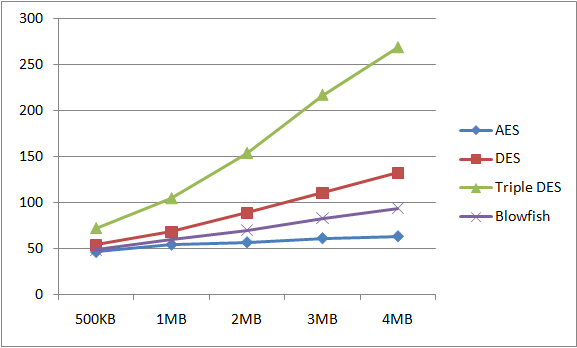
\includegraphics[scale=0.8]{images/alg_graf_1.png}
	\caption{Titkosítási idő (milliszekundum, függőleges) - fájlméret (vízszintes) grafikon.}
	\label{fig:alg_titkositas_graf}
\end{figure}

\begin{figure}[h]
	\centering
	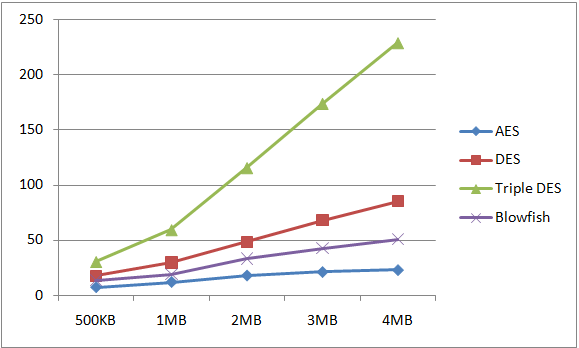
\includegraphics[scale=0.8]{images/alg_graf_2.png}
	\caption{Visszafejtési idő (milliszekundum, függőleges) - fájlméret (vízszintes) grafikon.}
	\label{fig:alg_visszafejtes_graf}
\end{figure}


\newpage \noindent  A 64 MB-os esetet külön diagramba rajzoltam, különben összenyomta volna az előző diagramokat:
\begin{figure}[h]
	\centering
	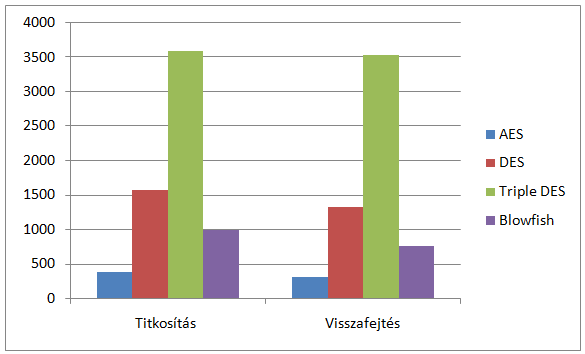
\includegraphics[scale=0.8]{images/alg_graf_3.png}
	\caption{64MB-os fájl titkosítás, visszafejtés. Függőleges tengely - idő (ms)}
	\label{fig:alg_64mb_graf}
\end{figure}

\vspace{25pt} \noindent \underline{Aszimmetrikus titkosítási algoritmusok:}
\vspace{15pt} \\ \textbf{RSA}
\vspace{5pt} \\ Szerettem volna a szimmetrikus algoritmusokkal összehasonlítani, de nem lenne korrekt, mivel az adatmennyiség felsőhatára, amit a javax.crypto könyvtár használatával titkosítani tudtam, az 245 byte volt. Ha nagyobb mérettel próbálkoztam ugyanazt a hibaüzenetet kaptam „Data must not be longer than 245 bytes”.
\vspace{5pt} \\Ezután az interneten jobban utána olvastam a problémának és megtudtam, hogy az RSA algoritmus maximum akkora mennyiségű adatot képes titkosítani, mint az RSA kulcs mérete (mínusz az ún. header data, azaz fejlécadat). 
\vspace{5pt} \\Kettő hatványait használtam kulcsméret megadására, először 2048 bit nagyságú kulccsal kezdtem. A következő mérések ezzel készültek (szintén milliszekundumban értendők az értékek):

\begin{center}
	\begin{tabular}{|p{2.4cm}|p{2cm}|p{2cm}|p{2cm}|p{2cm}|}
		\hline
		\textbf{Titkosítás} \newline \textbf{RSA} & \textbf{64 byte} & \textbf{128 byte} & \textbf{245 byte}\\
		\hline
		\textbf{1.mérés} & 28 & 24 & 28\\
		\hline
		\textbf{2.mérés} & 28 & 24 & 30\\
		\hline
		\textbf{3.mérés} & 25 & 26 & 30\\
		\hline
		\textbf{4.mérés} & 23 & 26 & 28\\
		\hline
		\textbf{5.mérés} & 24 & 25 & 28\\
		\hline
		\textbf{6.mérés} & 26 & 21 & 25\\
		\hline
		\textbf{7.mérés} & 27 & 23 & 22\\
		\hline
		\textbf{8.mérés} & 30 & 28 & 22\\
		\hline
		\textbf{9.mérés} & 29 & 26 & 21\\
		\hline
		\textbf{10.mérés} & 25 & 28 & 25\\
		\hline
		\hline
		\textbf{Átlag} & \textbf{26,5} & \textbf{25,1} & \textbf{25,9}\\
		\hline
	\end{tabular}
\end{center}

\begin{center}
	\begin{tabular}{|p{2.4cm}|p{2cm}|p{2cm}|p{2cm}|p{2cm}|}
		\hline
		\textbf{Visszafejtés} \newline \textbf{RSA} & \textbf{64 byte} & \textbf{128 byte} & \textbf{245 byte}\\
		\hline
		\textbf{1.mérés} & 7 & 6 & 7\\
		\hline
		\textbf{2.mérés} & 6 & 5 & 4\\
		\hline
		\textbf{3.mérés} & 6 & 7 & 5\\
		\hline
		\textbf{4.mérés} & 4 & 7 & 7\\
		\hline
		\textbf{5.mérés} & 6 & 7 & 6\\
		\hline
		\textbf{6.mérés} & 7 & 4 & 4\\
		\hline
		\textbf{7.mérés} & 5 & 7 & 9\\
		\hline
		\textbf{8.mérés} & 7 & 7 & 5\\
		\hline
		\textbf{9.mérés} & 8 & 5 & 7\\
		\hline
		\textbf{10.mérés} & 7 & 8 & 6\\
		\hline
		\hline
		\textbf{Átlag} & \textbf{6,3} & \textbf{6,3} & \textbf{6}\\
		\hline
	\end{tabular}
\end{center}

Ezután megpróbáltam nagyobb fájlokat titkosítani, így növelnem kellett a kulcs nagyságát is.
\vspace{5pt} \\ A kulcs nagysága: 8192 bit. Titkosítandó fájl nagysága: 1013 byte (a fejlécadat nagysága miatt ez lett a limit, de a kettőt összeadva egyébként $2^{10}$-en, azaz 1024 byte). Titkosított fájl mérete: 1024 byte.

\begin{center}
	\begin{tabular}{|p{2.4cm}|p{2.4cm}|p{2.4cm}|}
		\hline
		\textbf{1024 byte} & \textbf{Titkosítás} & \textbf{Visszafejtés}\\
		\hline
		\textbf{1.mérés} & 28 & 117\\
		\hline
		\textbf{2.mérés} & 21 & 123\\
		\hline
		\textbf{3.mérés} & 22 & 121\\
		\hline
		\textbf{4.mérés} & 31 & 121\\
		\hline
		\textbf{5.mérés} & 29 & 125\\
		\hline
		\textbf{6.mérés} & 23 & 119\\
		\hline
		\textbf{7.mérés} & 24 & 122\\
		\hline
		\textbf{8.mérés} & 27 & 121\\
		\hline
		\textbf{9.mérés} & 28 & 119\\
		\hline
		\textbf{10.mérés} & 23 & 124\\
		\hline
		\hline
		\textbf{Átlag} & \textbf{25,6} & \textbf{121,1}\\
		\hline
	\end{tabular}
\end{center}


\noindent Annak ellenére, hogy ezek az értékek nem  tűnnek nagynak, a számítógépemnek elég sokáig tartott minden mérés elvégzése, volt néhol 10 másodperc is, mire az eredményt megkaptam. Az említett ’System.currentTimeMillis()’ metódus használatát ajánlották az interneten kód futásidejének mérésére, így nem tudom mi lehetett a probléma, de mivel már az 1 kb-os fájl titkosítása eddig tartott, nagyobb fájlmérettel nem próbálkoztam.
\begin{figure}[h]
	\centering
	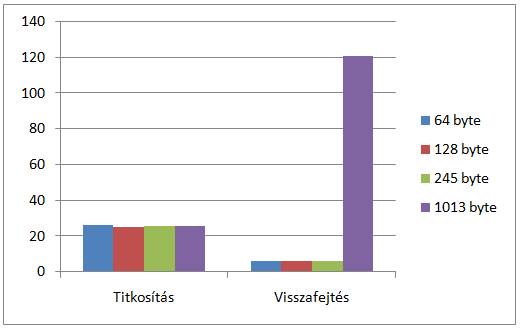
\includegraphics[scale=0.8]{images/alg_graf_4.png}
	\caption{RSA titkosítás, visszafejtés. Függőleges tengely - idő (ms)}
	\label{fig:rsa_graf}
\end{figure}
\\ \noindent DSA mérését és összehasonlítását nem tartom korrektnek, mivel nem nagy méretű adat titkosítására, hanem digitális aláírásokra lett kifejlesztve.
\\ECC mérést szintén nem készítettem, mivel nem tudtam. Utánanéztem az interneten és ECC titkosítást elméletileg a javax.crypto könyvtár segítségével nem lehet végrehajtani. Más függvény könyvtárat azért nem használtam, mert úgy gondolom fennáll a lehetősége, hogy eltérnek az algoritmusok implementálásai, így olyan könyvtár használata lenne optimális, amely az összes vizsgált algoritmust tartalmazza.



\vspace{15pt}\noindent Röviden összefoglalva, a tesztekkel és mérésekkel olyan eredményeket kaptam, amikre számítottam, annak ellenére, hogy a sebességük az előző alfejezetek leírásaiban nem lett számszerűsítve. 
\\Az AES-nél nem értek egyet a talált állítással, miszerint "Hátránya, hogy szoftveresen nehezen implementálható lehet, illetve komplexitása és nagysága miatt teljesítményi ideje is nagy lehet".
\\A szoftveres implementálás függvény könyvtár használata miatt volt egyszerű, a matematikai részét nem nekem kellett megoldanom.
\\Nagy teljesítményi ideje pedig relatív, hiszen a többi vizsgált szimmetrikus algoritmushoz képest az AES-é volt a legkisebb.